\section{Introduction}
You know how it works now....

\section{Methods}

Figure \ref{2-fig:sites} is a map and it's great.

\begin{figure}[htbp]
    \centering
    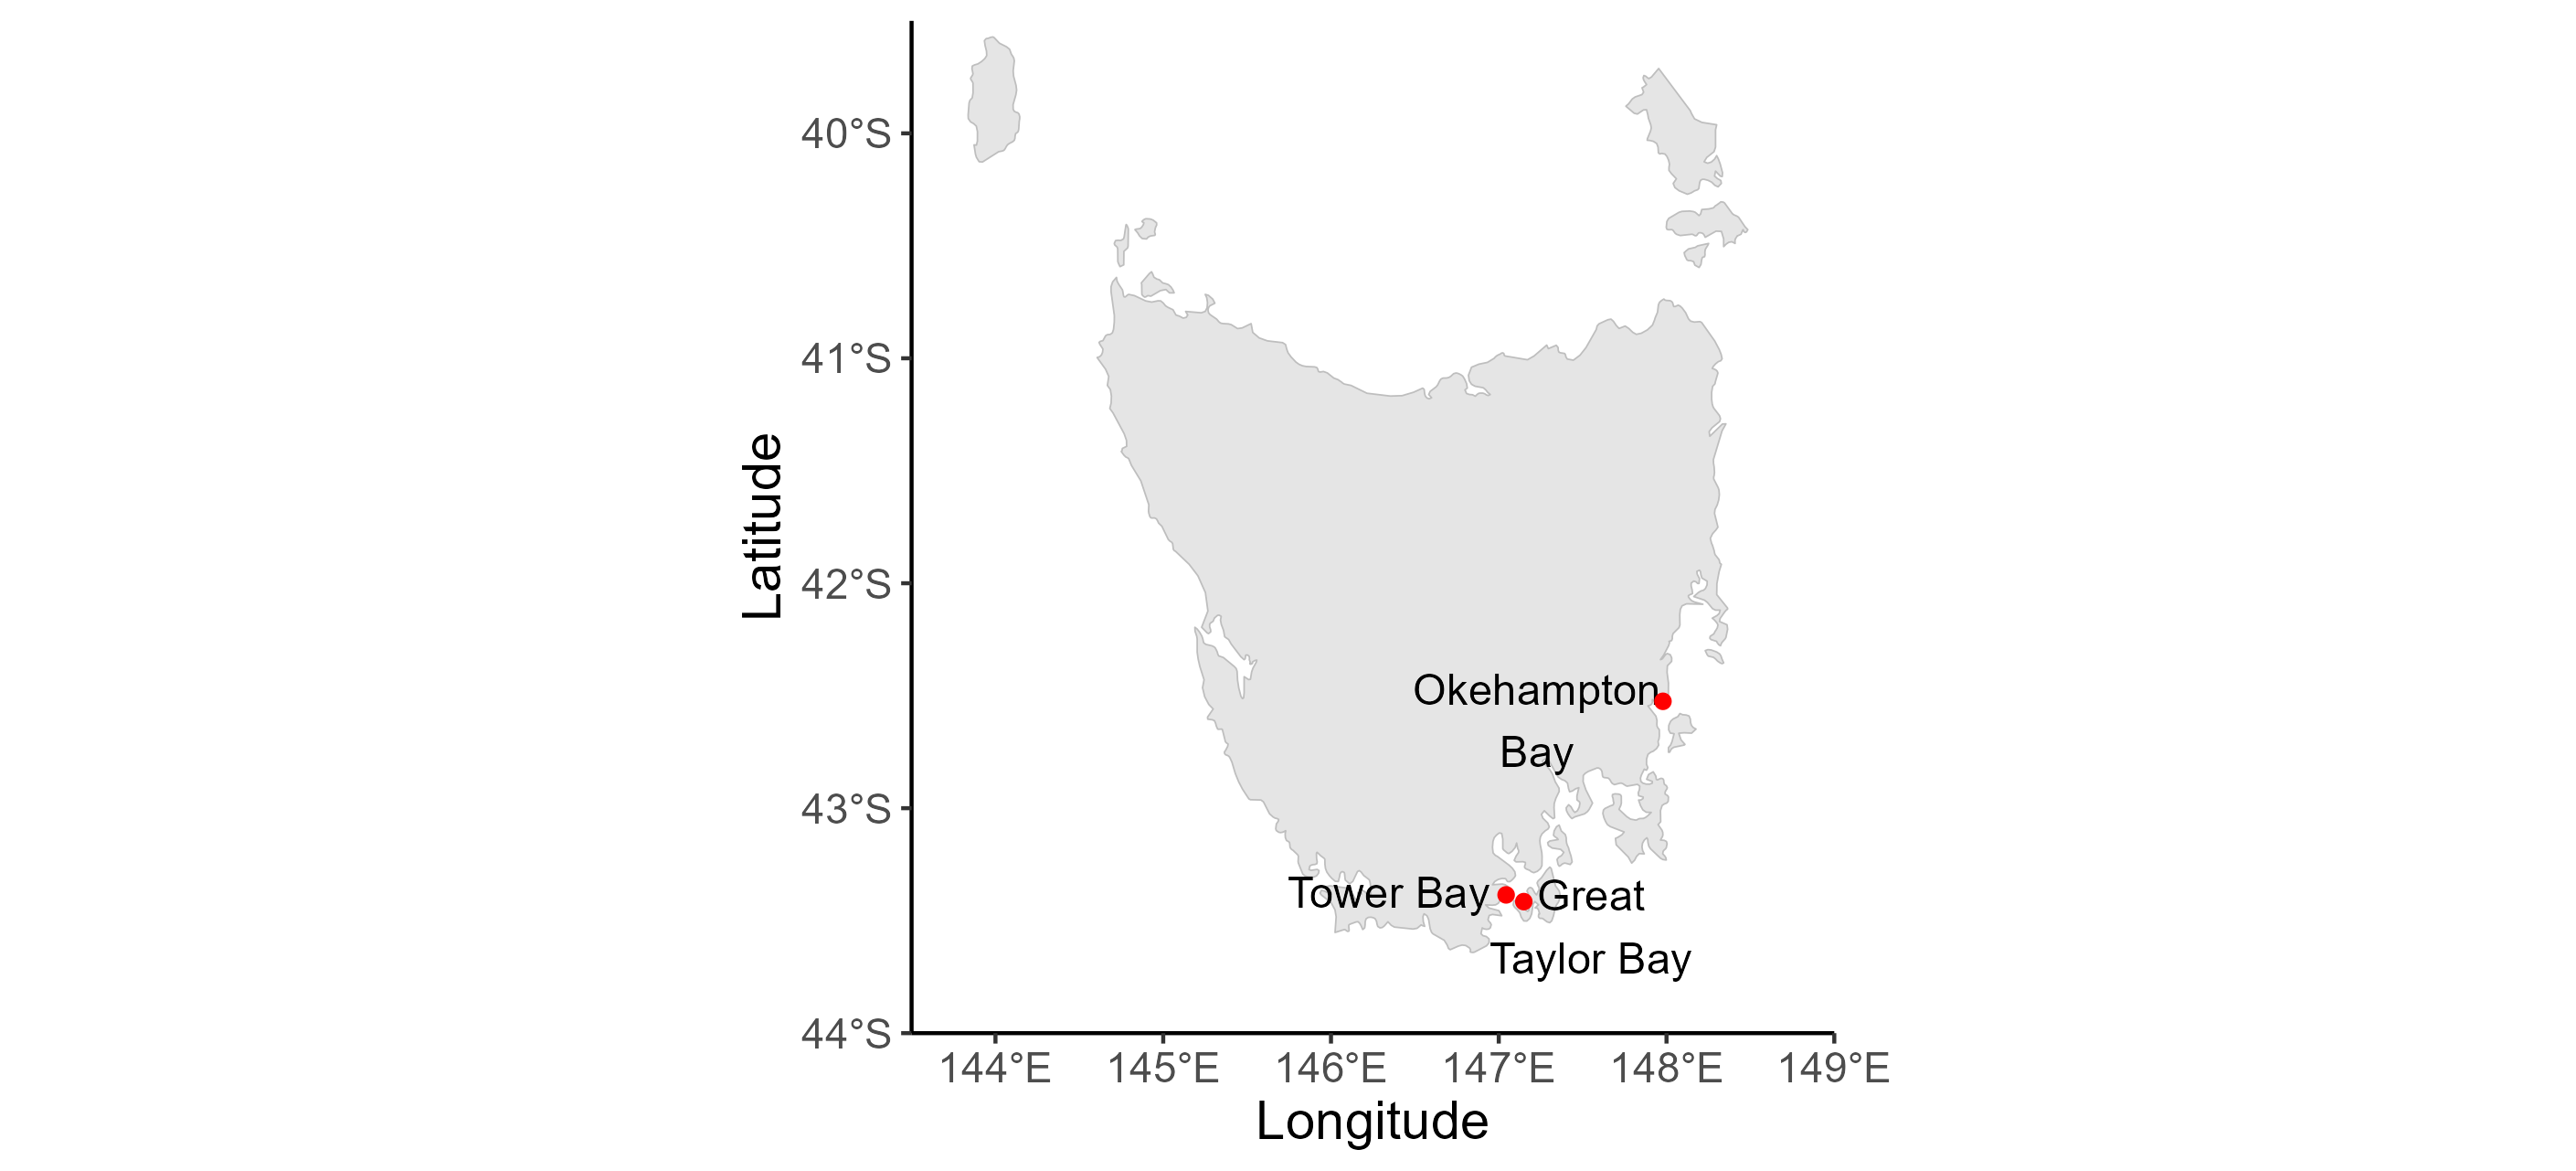
\includegraphics[width=0.85\linewidth, trim={4cm 0cm 4cm 0cm}, % trim={left bottom right top}
        clip]{figures/C2_1st_data_chapter/map.png}
    \caption[
        The three field sites from which my data was collected
    ]{
        The three field sites from which my data was collected. Adapted from \citet{biancacci_optimisation_2022}.
    } \label{2-fig:sites}
\end{figure}

\subsubsection{Experimental setup}
This new paragraph shows how to set \index{index items}index items
and \index{index items!subindex items} subindex items.

\subsection{Data collection and analysis}
I used the ``input'' command to put a big table in here because otherwise it takes up a lot of room in my code.
You can also try putting this table in landscape mode, but your text can't flow around it like a figure. 

%\begin{landscape}
    {\centering \small
\begin{longtable}{c l p{0.42\linewidth} r r r}
    \caption[
        A very fancy table
    ]{
        Summary of things! This table will span across multiple pages automatically, so that's nice. It will also place the top and bottom lines automatically at the page breaks.
    } \label{2-tab:summary} \\
    %
    \toprule
    Method & Unit & Description & Group 1 & Group 2 & Group 3 \\
    \midrule
    \endfirsthead
    %
    \caption[]{Notice that this caption is different than the first one. I like to replace the (usually long) first caption with a simple ``Table \thetable\ cont.''} \\
    %
    \toprule
    Symbol & Unit & Description & Group 1 & Group 2 & Group 3 \\
    \midrule
    \endhead
    %
    \bottomrule \endfoot
    \bottomrule \endlastfoot
    %
    % Start of main table
     & unit & This description is long. This column stays the same width, but the others will adjust to their contents. 
        & 100\footnote{\citet{smart_seasonal_2022}\label{smart2010}} 
        & 200\footref{smart2010}
        & 300\footref{smart2010} \\
    $B_a$ & unit & This description is long. This column stays the same width, but the others will adjust to their contents. 
        & 100\footnote{\citet{kopczak_variability_1994}\label{kopczak1994}} 
        & 200\footref{kopczak1994}
        & 300\footnote{\citet{miller_ecophysiology_2003}\label{miller2003}} \\
    $C_a$ & unit & This description is long. This column stays the same width, but the others will adjust to their contents.  
        & 100\footref{miller2003}
        & 200\footnote{\citet{wickham_species-specific_2019}\label{wickham2019}}
        & 300\footref{kopczak1994} \\
    $D_a$ & unit & This description is long. This column stays the same width, but the others will adjust to their contents.  
        & 100\footnote{\citet{zuniga_seasonal_2020}\label{zuniga2020}}
        & 200\footref{wickham2019}
        & 300\footref{zuniga2020} \\
    $E_a$ & unit & This description is long. This column stays the same width, but the others will adjust to their contents.  
        & 100\footref{zuniga2020} 
        & 200\footref{miller2003}
        & 300\footref{zuniga2020} \\
    $F_a$ & unit & This description is long. This column stays the same width, but the others will adjust to their contents.  
        & 100\footref{miller2003}
        & 200\footnote{\citet{trancoso_modelling_2005}\label{trancoso2005}}
        & 300\footref{trancoso2005} \\
    $G_a$ & unit & This description is long. This column stays the same width, but the others will adjust to their contents. 
        & 100\footnote{\citet{wheeler_effect_1980}\label{wheeler1980}}
        & 200\footref{trancoso2005} 
        & 300\footnote{\citet{biancacci_optimisation_2022}\label{biancacci2022}} \\
    $H_a$ & unit & This description is long. This column stays the same width, but the others will adjust to their contents.  
        & 100\footnote{\citet{enriquez_light_1994}\label{enriquez1994}}
        & 200\footref{biancacci2022} 
        & 300\footref{zuniga2020} \\
    $I_a$ & unit & This description is long. This column stays the same width, but the others will adjust to their contents.   
        & 100\footnote{\citet{gao_growth_2016}\label{gao2016}}
        & 200\footnote{\citet{buschmann_opportunities_2008}}
        & 300\footref{gao2016} \\ 
    $J_a$ & unit & This description is long. This column stays the same width, but the others will adjust to their contents.  
        & 100\footref{wickham2019}
        & 200\footnote{\citet{zimmerman_episodic_1984, zimmerman_situ_1986}}
        & 300\footnote{\citet{bearham_temperature_2013}} \\
    $K_a$ & unit & This description is long. This column stays the same width, but the others will adjust to their contents. 
        & 100\footnote{See section \ref{chap:3rd-data}\label{igiveup}}
        & 200\footnote{\citet{fernandez_nitrogen_2020}\label{fernandez2020}}
        & 300\footnote{\citet{tala_growth_2005}\label{tala2005}} \\* % I've decided I don't want the page break to happen here.
    $L_a$ & unit & This description is long. This column stays the same width, but the others will adjust to their contents.  
        & 100\footref{biancacci2022} 
        & 200\footnote{\citet{bolton_temperature_1987}\label{bolton1987}}
        & 300\footref{trancoso2005} \\
    $M_a$ & unit & This description is long. This column stays the same width, but the others will adjust to their contents.  
        & 100\footref{gao2016}  
        & 200\footref{smart2010}
        & 300\footnote{\citet{james_thermal_2023}\label{james2023}} \\
    $N_a$ & unit & This description is long. This column stays the same width, but the others will adjust to their contents.  
        & 100\footref{james2023}  
        & 200\footref{bolton1987}  
        & 300\footnote{\citet{hernandez-carmona_effect_2001}\label{hernandez2001}} \\
    $O_a$ & unit & This description is long. This column stays the same width, but the others will adjust to their contents.  
        & 100\footref{miller2003}
        & 200\footnote{\citet{staehr_physiological_2009}}
        & 300\footnote{\citet{mabin_physiological_2019}\label{mabin2019}} \\
    $P_a$ & unit & This description is long. This column stays the same width, but the others will adjust to their contents.  
        & 100\footref{mabin2019}  
        & 200\footref{hernandez2001}  
        & 300\footref{smart2010} \\
    $Q_a$ & unit & This description is long. This column stays the same width, but the others will adjust to their contents.  
        & 100\footref{biancacci2022} 
        & 200\footref{wickham2019}
        & 300\footref{bolton1987} \\
    $R_a$ & unit & This description is long. This column stays the same width, but the others will adjust to their contents.  
        & 100\footref{smart2010}
        & 200\footref{smart2010}
        & 300\footref{gao2016} \\
    $S_a$ & unit & This description is long. This column stays the same width, but the others will adjust to their contents.  
        & 100\footref{mabin2019}  
        & 200\footref{james2023}  
        & 300\footref{zuniga2020} \\
    $T_a$ & unit & This description is long. This column stays the same width, but the others will adjust to their contents.  
        & 100\footref{zuniga2020} 
        & 200\footref{trancoso2005} 
        & 300\footref{hernandez2001} \\
    $U_a$ & unit & This description is long. This column stays the same width, but the others will adjust to their contents.  
        & 100\footref{hernandez2001}  
        & 200\footref{tala2005}  
        & 300\footref{wickham2019} \\
\end{longtable}
}
%\end{landscape}

\section{Results}

\subsection{Subset 1}

Sometimes subfigures are needed, and you can do it with Figures \ref{2-fig:parrots}A \& B.
However, you might just output the figures from R with the As and Bs already on them and put them in here as-is. 

\begin{figure}[hbtp]
    \centering
    \begin{overpic}[width=0.48\linewidth, trim={1.5cm 0cm 1cm 0cm}, clip%,grid, tics = 10
        ]{figures/C2_1st_data_chapter/parrots.jpg}
        \put(-5,65) {\normalsize\textbf{A}}
    \end{overpic}
    \begin{overpic}[width=0.48\linewidth, trim={1.5cm 0cm 1cm 0cm}, clip%,grid, tics = 10
        ]{figures/C2_1st_data_chapter/parrots.jpg}
        \put(-5,65) {\normalsize\textbf{B}}
    \end{overpic}
    \begin{overpic}[width=0.97\linewidth, trim={0cm 0cm 0cm -0.1cm}, clip%, grid, tics = 5
        ]{figures/C2_1st_data_chapter/parrots.jpg}
        \put(-2.5,57.5) {\normalsize\textbf{C}}
    \end{overpic}
    \caption[
        Example of sub-figures
    ]{
        Sub-figures can be put side-by-side, and you can use trimming and grids to get the sizing and scaling right.
    }\label{2-fig:parrots}
\end{figure}

\subsection{Subset 2}

\begin{landscape}
\begin{figure}[p]
    \centering
    %
    \begin{overpic}[width=0.4\linewidth%, grid, tics = 10 
                    , trim={-2.5cm 2.5cm 0cm -0.5cm} % left bottom right top
                    , clip
        ]{figures/C2_1st_data_chapter/liopleurodon.jpg}
        \put (-6, 55) {\normalsize\textbf{A}}
    \end{overpic}
    %
    \begin{overpic}[width=0.4\linewidth%, grid, tics = 10
                    , trim={-2.5cm 2.5cm 0cm -0.5cm} % left bottom right top
                    , clip
        ]{figures/C2_1st_data_chapter/liopleurodon.jpg}
        \put (-6, 55) {\normalsize\textbf{B}}
    \end{overpic}
    %
    \begin{overpic}[width=0.4\linewidth%, grid, tics = 10
                    , trim={-2.5cm 2.5cm 0cm -0.5cm} % left bottom right top
                    , clip
        ]{figures/C2_1st_data_chapter/liopleurodon.jpg}
        \put (-6, 55) {\normalsize\textbf{C}}
    \end{overpic}
    %
    \begin{overpic}[width=0.4\linewidth%, grid, tics = 10
                    , trim={-2.5cm 2.5cm 0cm -0.5cm} % left bottom right top
                    , clip
        ]{figures/C2_1st_data_chapter/liopleurodon.jpg}
        \put (-6, 55) {\normalsize\textbf{D}}
    \end{overpic}
    %
    \caption[IT'S A LIOPLEURODON CHARLIE]{Landscape, baby! You can trim and clip figures in Latex if you want to, although honestly it's a lot easier to do the subfigure layouts in ggplot2 and then just bring the whole picture into Latex.}
    \label{2-fig:liopleurodon}
    %
\end{figure}
\end{landscape}

\clearpage
\section{Discussion}
\subsection{I have so much to talk about}
\lipsum[1][]

\subsection{You can't shut me up}
\lipsum[3][]

\subsubsection{Just one more thing}
\lipsum[5][]
